\chapter{Smartphone}
\label{ch:smartphone}

\section{Introduction}

Dans votre poche se trouve un appareil qui a changé la vie de milliards de personnes partout dans le monde. Le troisième écran personnel (après la télévision et l’ordinateur) c'est le plus personnel de tous et la priorité clés des entreprises de cette décennie afin de proposer de nouveaux services.

Cependant le développement mobile est une activité plus difficile que le développement sur Pc. Les plateformes mobiles sont très fragmentées et les développeurs doivent travailler avec un minimum de ressources. Heureusement le web-mobile permet de traiter plus facilement cette fragmentation en offrant aux développeurs la possibilité de créer des applications qui s’éxecutent sur plus de plateformes qu’en natif.

Les statistiques les plus récentes, au moment de la rédaction de ce mémoire, indiquent que Android est en tête du classement des smartphones avec environ plus de 70\% de toutes les ventes au dernier trimestres 2012, iOS est à environ 20\% dans la même période. Blackberry un très grand nom dans le monde des smartphone ainsi que Windows Phone, Bada et Symbian avec d’autre plateformes plus ou moins connues, se partagent le reste des pourcentages restant.


\begin{center}
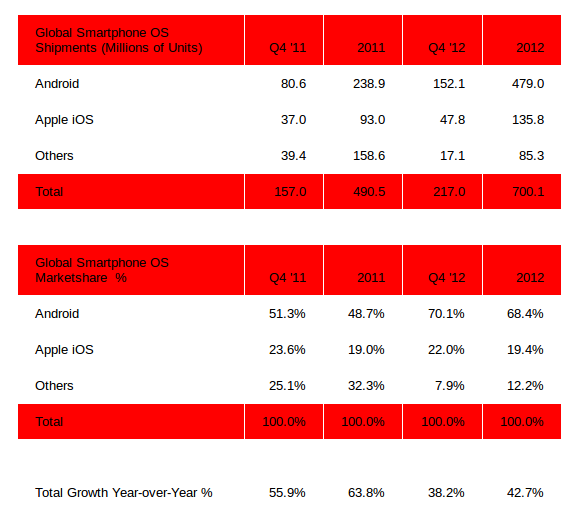
\includegraphics[width=14cm]{img/marche_smartphone.png}
\label{Parts de marché smartphone}
\end{center}

Ces chiffres montrent clairement que le marché des smartphones est très différent du marché des PC, il n’y a pas vraiment de gagnant et les societés voulant profiter ce nouveau canal de communication ont à faire d’importants investissement afin d’être présents dans autant de poches que possible. Beaucoup d’applications doivent être écrites dans au moins deux ou trois plateformes (généralement iOS, Android et Blackberry) pour atteindre une tranche non négligeable du marché.

Actuellement les smartphone ont conquis le marché des téléphones portables ces dernières années.

Beaucoup de choses ont changé depuis 2007, mais comme comme pour son homologue de bureau, le Web apparaît comme la solution multiplateforme la plus importante à la dispositions des développeurs d’aujourd’hui.

\subsection{La croissance du Web mobiles}

Une des avancées de cette nouvelle génération d’appareils mobiles est la possibilité d’utiliser pleinement un véritable navigateur Web mobile, compatible avec la plupart des normes actuelles telles que HTML5, CSS, JavaScript et de nombreux autres standards.

Beaucoup d’entre nous se souviennent d'avoir regardé Steve Jobs présentant les capacités du navigateur Safari mobile dans le premier iPhone, tout en reconnaissant qu’une nouvelle ère avait commencé précisément ce jour-là.

Les navigateurs mobiles n'étaient pas seulement aussi capable que leurs homologues de bureau, ils étaient meilleurs que les pc , ils étaient rapides et étaient entièrement conformes aux normes.

La montée en puissance de l’internet mobile a apporté de nouvelles possibilités, en particulier dans les pays à faible pénétration technologique comme l’Amérique latine ou l’Afrique. Les smartphone apparaissent alors comme un bien beaucoup moins cher pour accéder aux informations et services en ligne.

Exemple, en 2010, plus de 30\% des accès web en provenance de l’Afrique était réalisés à partir d’un smartphone.

Dans le monde, on estime que plus de 50\% de toutes les requêtes web viendront d’appareils mobile d’ici 2015.

\subsection{Nouveaux paradigmes}

Tout cela représente un énorme changement dans notre façon de développer des logiciels.

Un changement radical indiquant que le web mobile est en train de devenir le nouveau canal principal de la présence du web. L’utilisation de la bande passante à partir d’un pc va être inférieure à celle du mobile.

Mais cette nouvelle perspective pose quelques questions:

\begin{itemize}

  \item
  Combien de plateformes dois-je tester pour mon site web?

  \item
  Dois-je me soucier des téléphones mobiles bas de gamme?

  \item
  Quelles bibliothèques puis-je utiliser pour accélérer mon développement?

  \item
  Quel est le niveau de support des standard dans les principaux navigateurs mobiles.

\end{itemize}
Pour ce faire, nous allons étudier les technologies suivantes, qui sont actuellement très prometteuses et qui ont une feuille de route très interessantes


\begin{itemize}

  \item[\textbullet]
  PhoneGap

  \item[\textbullet]
  Sencha Touch

  \item[\textbullet]
  Jquery Mobile

\end{itemize}

Il y a bien sur d’autres technologies intéressantes mais je vais me limiter à l’étude de ces 3 frameworks.